% Options for packages loaded elsewhere
\PassOptionsToPackage{unicode}{hyperref}
\PassOptionsToPackage{hyphens}{url}
\PassOptionsToPackage{dvipsnames,svgnames*,x11names*}{xcolor}
%
\documentclass[
]{article}
\usepackage{lmodern}
\usepackage{amssymb,amsmath}
\usepackage{ifxetex,ifluatex}
\ifnum 0\ifxetex 1\fi\ifluatex 1\fi=0 % if pdftex
  \usepackage[T1]{fontenc}
  \usepackage[utf8]{inputenc}
  \usepackage{textcomp} % provide euro and other symbols
\else % if luatex or xetex
  \usepackage{unicode-math}
  \defaultfontfeatures{Scale=MatchLowercase}
  \defaultfontfeatures[\rmfamily]{Ligatures=TeX,Scale=1}
\fi
% Use upquote if available, for straight quotes in verbatim environments
\IfFileExists{upquote.sty}{\usepackage{upquote}}{}
\IfFileExists{microtype.sty}{% use microtype if available
  \usepackage[]{microtype}
  \UseMicrotypeSet[protrusion]{basicmath} % disable protrusion for tt fonts
}{}
\makeatletter
\@ifundefined{KOMAClassName}{% if non-KOMA class
  \IfFileExists{parskip.sty}{%
    \usepackage{parskip}
  }{% else
    \setlength{\parindent}{0pt}
    \setlength{\parskip}{6pt plus 2pt minus 1pt}}
}{% if KOMA class
  \KOMAoptions{parskip=half}}
\makeatother
\usepackage{xcolor}
\IfFileExists{xurl.sty}{\usepackage{xurl}}{} % add URL line breaks if available
\IfFileExists{bookmark.sty}{\usepackage{bookmark}}{\usepackage{hyperref}}
\hypersetup{
  pdftitle={Machine learning Data Competition 2020},
  pdfauthor={Shreyasvi Natraj},
  colorlinks=true,
  linkcolor=Maroon,
  filecolor=Maroon,
  citecolor=Blue,
  urlcolor=blue,
  pdfcreator={LaTeX via pandoc}}
\urlstyle{same} % disable monospaced font for URLs
\usepackage[margin=1in]{geometry}
\usepackage{color}
\usepackage{fancyvrb}
\newcommand{\VerbBar}{|}
\newcommand{\VERB}{\Verb[commandchars=\\\{\}]}
\DefineVerbatimEnvironment{Highlighting}{Verbatim}{commandchars=\\\{\}}
% Add ',fontsize=\small' for more characters per line
\usepackage{framed}
\definecolor{shadecolor}{RGB}{248,248,248}
\newenvironment{Shaded}{\begin{snugshade}}{\end{snugshade}}
\newcommand{\AlertTok}[1]{\textcolor[rgb]{0.94,0.16,0.16}{#1}}
\newcommand{\AnnotationTok}[1]{\textcolor[rgb]{0.56,0.35,0.01}{\textbf{\textit{#1}}}}
\newcommand{\AttributeTok}[1]{\textcolor[rgb]{0.77,0.63,0.00}{#1}}
\newcommand{\BaseNTok}[1]{\textcolor[rgb]{0.00,0.00,0.81}{#1}}
\newcommand{\BuiltInTok}[1]{#1}
\newcommand{\CharTok}[1]{\textcolor[rgb]{0.31,0.60,0.02}{#1}}
\newcommand{\CommentTok}[1]{\textcolor[rgb]{0.56,0.35,0.01}{\textit{#1}}}
\newcommand{\CommentVarTok}[1]{\textcolor[rgb]{0.56,0.35,0.01}{\textbf{\textit{#1}}}}
\newcommand{\ConstantTok}[1]{\textcolor[rgb]{0.00,0.00,0.00}{#1}}
\newcommand{\ControlFlowTok}[1]{\textcolor[rgb]{0.13,0.29,0.53}{\textbf{#1}}}
\newcommand{\DataTypeTok}[1]{\textcolor[rgb]{0.13,0.29,0.53}{#1}}
\newcommand{\DecValTok}[1]{\textcolor[rgb]{0.00,0.00,0.81}{#1}}
\newcommand{\DocumentationTok}[1]{\textcolor[rgb]{0.56,0.35,0.01}{\textbf{\textit{#1}}}}
\newcommand{\ErrorTok}[1]{\textcolor[rgb]{0.64,0.00,0.00}{\textbf{#1}}}
\newcommand{\ExtensionTok}[1]{#1}
\newcommand{\FloatTok}[1]{\textcolor[rgb]{0.00,0.00,0.81}{#1}}
\newcommand{\FunctionTok}[1]{\textcolor[rgb]{0.00,0.00,0.00}{#1}}
\newcommand{\ImportTok}[1]{#1}
\newcommand{\InformationTok}[1]{\textcolor[rgb]{0.56,0.35,0.01}{\textbf{\textit{#1}}}}
\newcommand{\KeywordTok}[1]{\textcolor[rgb]{0.13,0.29,0.53}{\textbf{#1}}}
\newcommand{\NormalTok}[1]{#1}
\newcommand{\OperatorTok}[1]{\textcolor[rgb]{0.81,0.36,0.00}{\textbf{#1}}}
\newcommand{\OtherTok}[1]{\textcolor[rgb]{0.56,0.35,0.01}{#1}}
\newcommand{\PreprocessorTok}[1]{\textcolor[rgb]{0.56,0.35,0.01}{\textit{#1}}}
\newcommand{\RegionMarkerTok}[1]{#1}
\newcommand{\SpecialCharTok}[1]{\textcolor[rgb]{0.00,0.00,0.00}{#1}}
\newcommand{\SpecialStringTok}[1]{\textcolor[rgb]{0.31,0.60,0.02}{#1}}
\newcommand{\StringTok}[1]{\textcolor[rgb]{0.31,0.60,0.02}{#1}}
\newcommand{\VariableTok}[1]{\textcolor[rgb]{0.00,0.00,0.00}{#1}}
\newcommand{\VerbatimStringTok}[1]{\textcolor[rgb]{0.31,0.60,0.02}{#1}}
\newcommand{\WarningTok}[1]{\textcolor[rgb]{0.56,0.35,0.01}{\textbf{\textit{#1}}}}
\usepackage{graphicx,grffile}
\makeatletter
\def\maxwidth{\ifdim\Gin@nat@width>\linewidth\linewidth\else\Gin@nat@width\fi}
\def\maxheight{\ifdim\Gin@nat@height>\textheight\textheight\else\Gin@nat@height\fi}
\makeatother
% Scale images if necessary, so that they will not overflow the page
% margins by default, and it is still possible to overwrite the defaults
% using explicit options in \includegraphics[width, height, ...]{}
\setkeys{Gin}{width=\maxwidth,height=\maxheight,keepaspectratio}
% Set default figure placement to htbp
\makeatletter
\def\fps@figure{htbp}
\makeatother
\setlength{\emergencystretch}{3em} % prevent overfull lines
\providecommand{\tightlist}{%
  \setlength{\itemsep}{0pt}\setlength{\parskip}{0pt}}
\setcounter{secnumdepth}{5}
\usepackage{booktabs}
\usepackage{longtable}
\usepackage{array}
\usepackage{multirow}
\usepackage{wrapfig}
\usepackage{float}
\usepackage{colortbl}
\usepackage{pdflscape}
\usepackage{tabu}
\usepackage{threeparttable}
\usepackage{threeparttablex}
\usepackage[normalem]{ulem}
\usepackage{makecell}
\usepackage{xcolor}

\title{Machine learning Data Competition 2020}
\usepackage{etoolbox}
\makeatletter
\providecommand{\subtitle}[1]{% add subtitle to \maketitle
  \apptocmd{\@title}{\par {\large #1 \par}}{}{}
}
\makeatother
\subtitle{Report I.}
\author{Shreyasvi Natraj}
\date{}

\begin{document}
\maketitle

\section{Introduction}

For the given data competition, we were provided with data pertaining to
previous adverstisement campaigns as well as demographics of users who
have been a part of the survey conducted.

For the objective of the given task, we are required to train a model
that can be used in order to predict whether if a user is likely to have
a ``conversion'' where a ``conversion'' refers to the user clicking on
the advertisement and subscribing to the service.

Since the data provided is used in order to predict a categorical
variable i.e.~``conversion/y'', we planned to use do a quick an dirty
implementation of the following models to check for their accuracy:

\emph{K-Nearest Neighbours }Random Forest \emph{LDA, QDA \& C5.0
}Supported Vector Machines *Logistic Regression

We initially carried out with exploratory data analysis for the data
provided to us by considering na values as NaN values.

\section{Exploratory data analysis}

We observed from this that it would not be a good idea to not consider
the na values as NaN but as a separate level. However, based on
similarity in between the classes, we can merge different levels of a
factor into lesser number of levels so they are easier for our model to
interpret.

\subsection{Interpretation}

We also carried out the same process of data analysis after converting
categorical variables into inteager format which tend to show a similar
fashion to the current analysis being carried out. However, we replaced
``na'' values with 0 which made the data much more consistent. We also
observed that \texttt{time\_spent},\texttt{outcome\_old} and \texttt{X3}
tends to hold a very high significance when predicting conversion
\texttt{y}.

\subsection{Data Distribution}

\begin{verbatim}
## Rows: 8,526
## Columns: 17
## $ age              <int> 35, 42, 38, 71, 37, 26, 27, 28, 57, 44, 34, 26, 33...
## $ job              <fct> manager, manager, industrial_worker, retired, unem...
## $ marital          <fct> single, married, married, married, single, married...
## $ education        <fct> grad_school, grad_school, university, high_school,...
## $ device           <fct> NA, smartphone, NA, smartphone, desktop, smartphon...
## $ day              <int> 30, 17, 14, 13, 27, 17, 30, 7, 26, 28, 12, 2, 6, 2...
## $ month            <int> 5, 7, 5, 11, 4, 7, 6, 5, 5, 12, 8, 12, 5, 5, 11, 2...
## $ time_spent       <dbl> 37.65, 39.25, 10.50, 8.80, 20.80, 57.00, 3.75, 10....
## $ banner_views     <int> 1, 1, 2, 2, 2, 3, 5, 1, 5, 1, 1, 1, 1, 2, 1, 2, 1,...
## $ banner_views_old <int> 0, 0, 0, 1, 3, 0, 0, 1, 0, 0, 0, 0, 3, 0, 0, 0, 5,...
## $ days_elapsed_old <int> -1, -1, -1, 98, 179, -1, -1, 339, -1, -1, -1, -1, ...
## $ outcome_old      <fct> NA, NA, NA, success, other, NA, NA, other, NA, NA,...
## $ X1               <int> 0, 0, 0, 0, 0, 1, 0, 0, 0, 0, 0, 0, 0, 1, 0, 0, 0,...
## $ X2               <int> 0, 0, 0, 0, 0, 0, 0, 0, 0, 0, 0, 0, 1, 0, 0, 0, 0,...
## $ X3               <int> 1, 1, 1, 0, 0, 1, 1, 1, 0, 0, 1, 0, 1, 1, 0, 0, 0,...
## $ X4               <dbl> 0.07793293, 0.07283969, 0.07607176, 0.09640840, 0....
## $ y                <int> 1, 1, 0, 1, 1, 1, 0, 0, 0, 1, 0, 1, 0, 0, 1, 0, 1,...
\end{verbatim}

\begin{figure}

{\centering 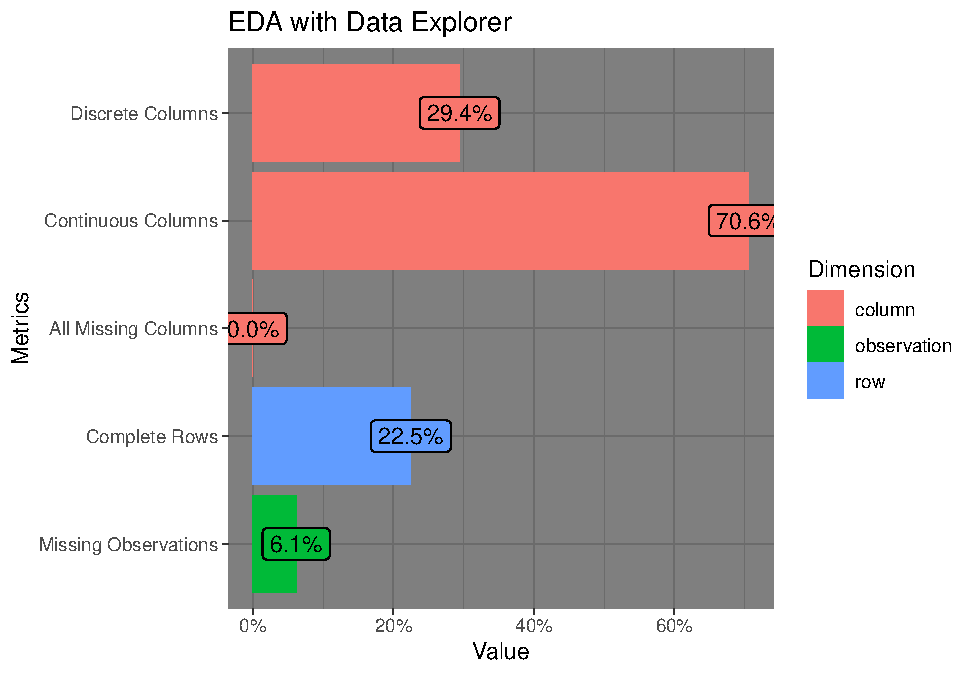
\includegraphics[width=0.75\linewidth]{report_files/figure-latex/Data Distribution-1} 

}

\caption{Data Distribution}\label{fig:Data Distribution}
\end{figure}
\subsection{Missing Columns}
\begin{figure}

{\centering 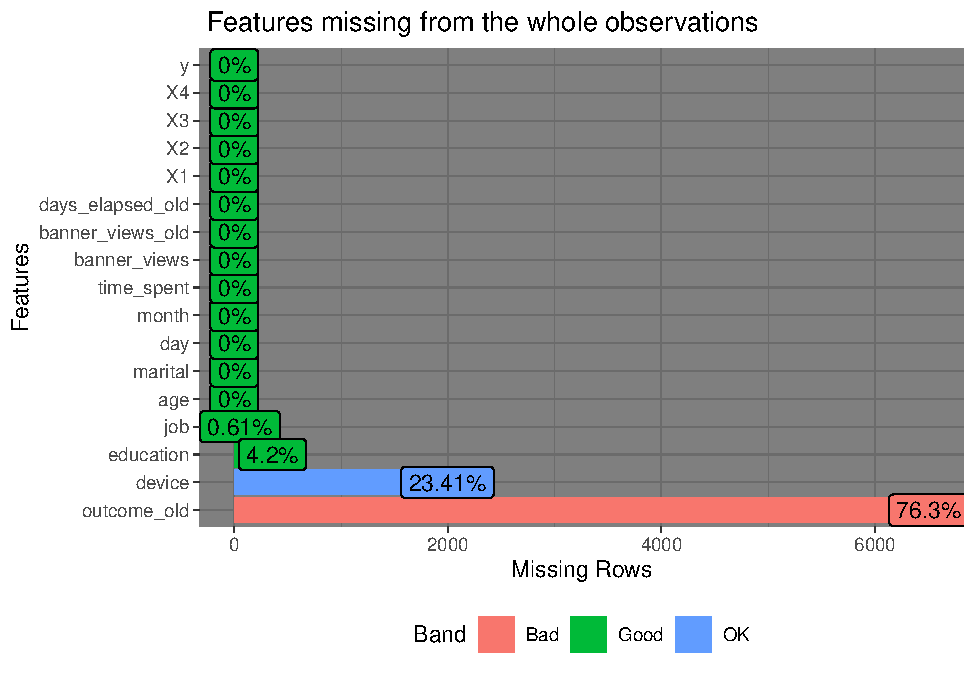
\includegraphics[width=0.75\linewidth]{report_files/figure-latex/Missing variables-1} 

}

\caption{Missing Columns}\label{fig:Missing variables}
\end{figure}
\subsection{EDA for Continuous variables}
\begin{figure}

{\centering 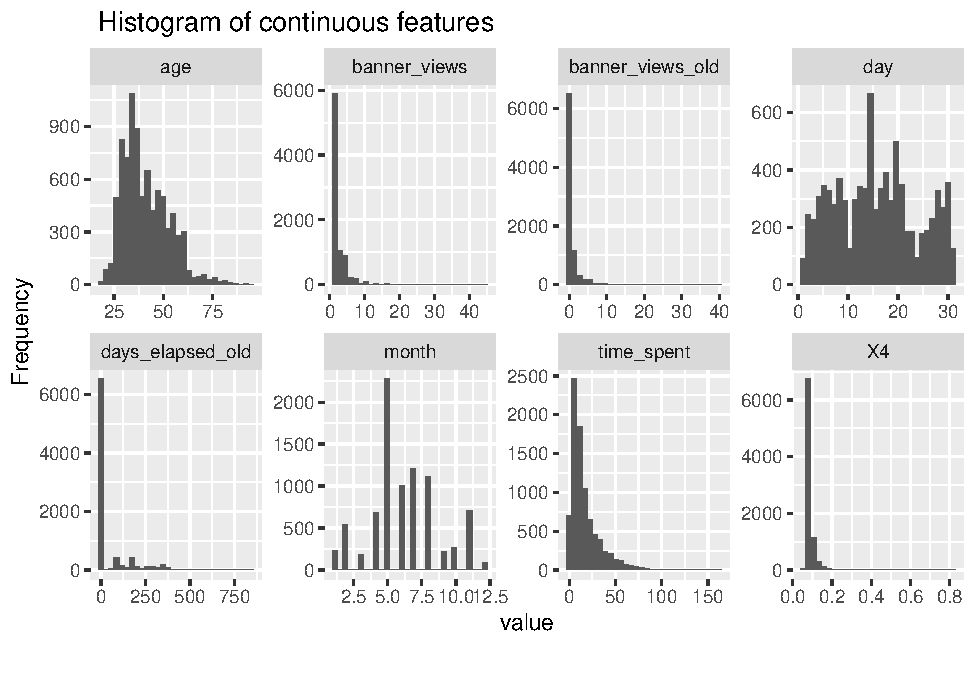
\includegraphics[width=0.75\linewidth]{report_files/figure-latex/Continous variables-1} 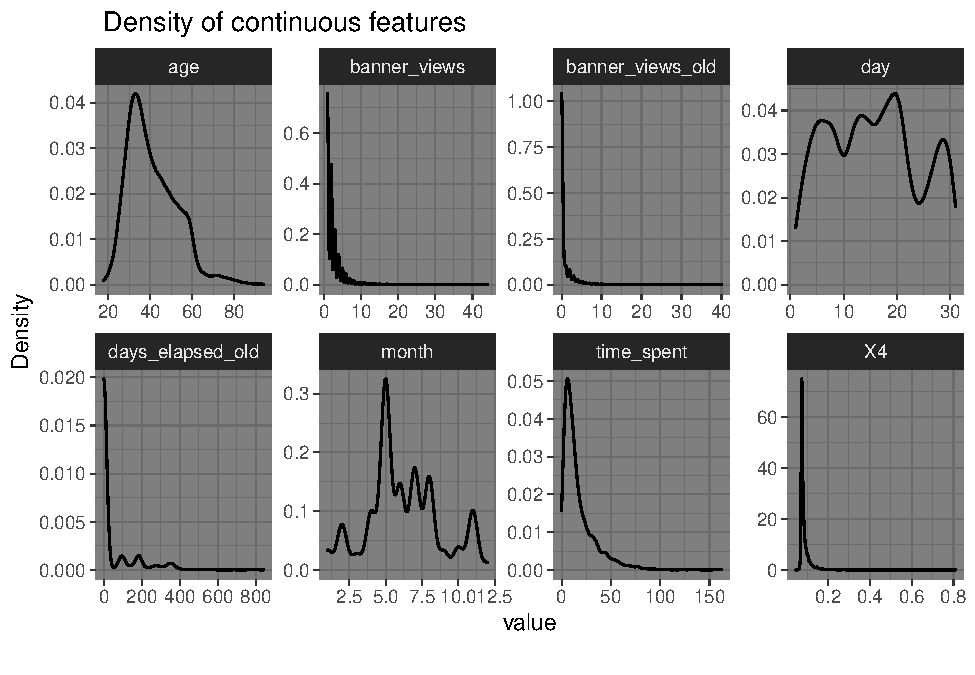
\includegraphics[width=0.75\linewidth]{report_files/figure-latex/Continous variables-2} 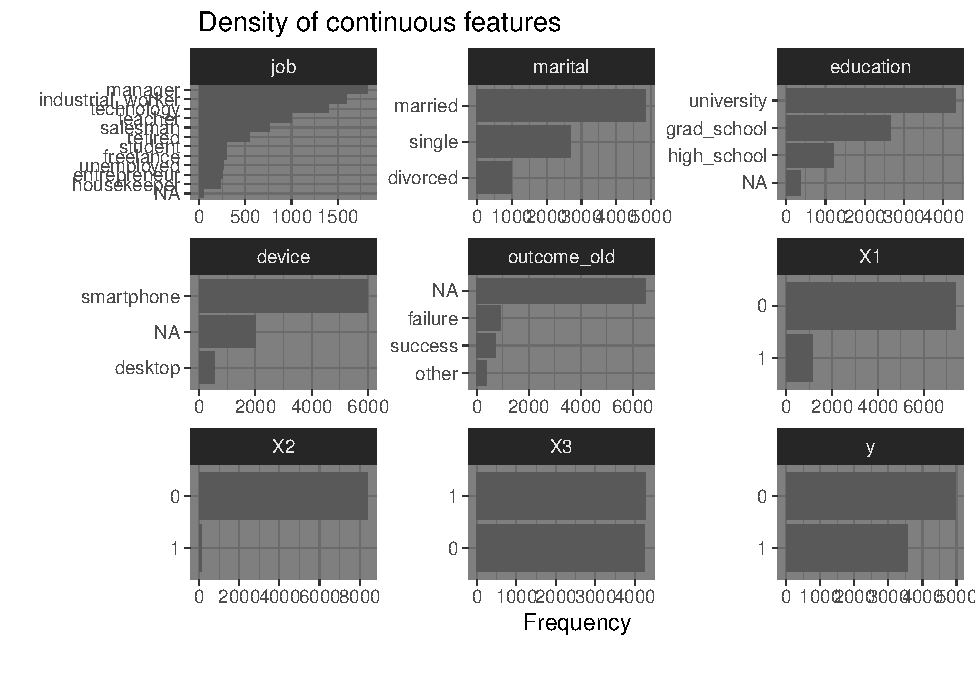
\includegraphics[width=0.75\linewidth]{report_files/figure-latex/Continous variables-3} 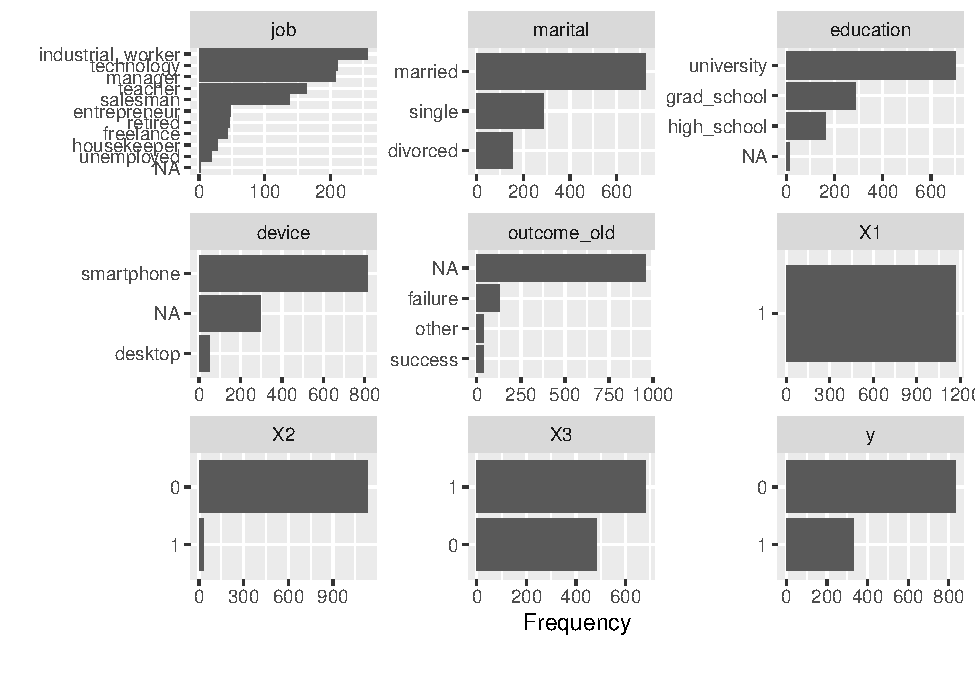
\includegraphics[width=0.75\linewidth]{report_files/figure-latex/Continous variables-4} 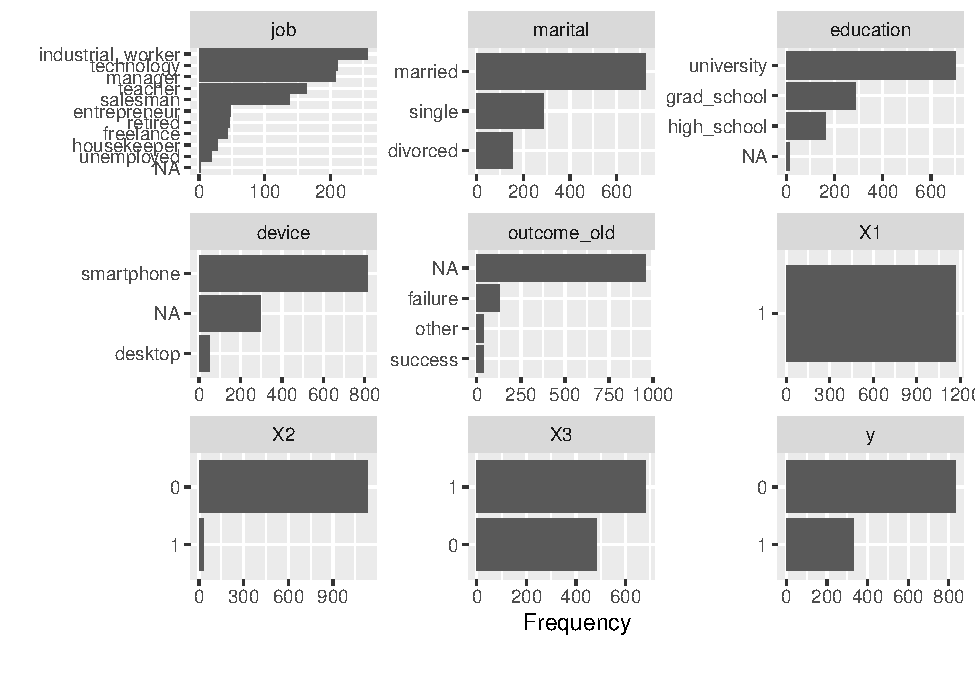
\includegraphics[width=0.75\linewidth]{report_files/figure-latex/Continous variables-5} 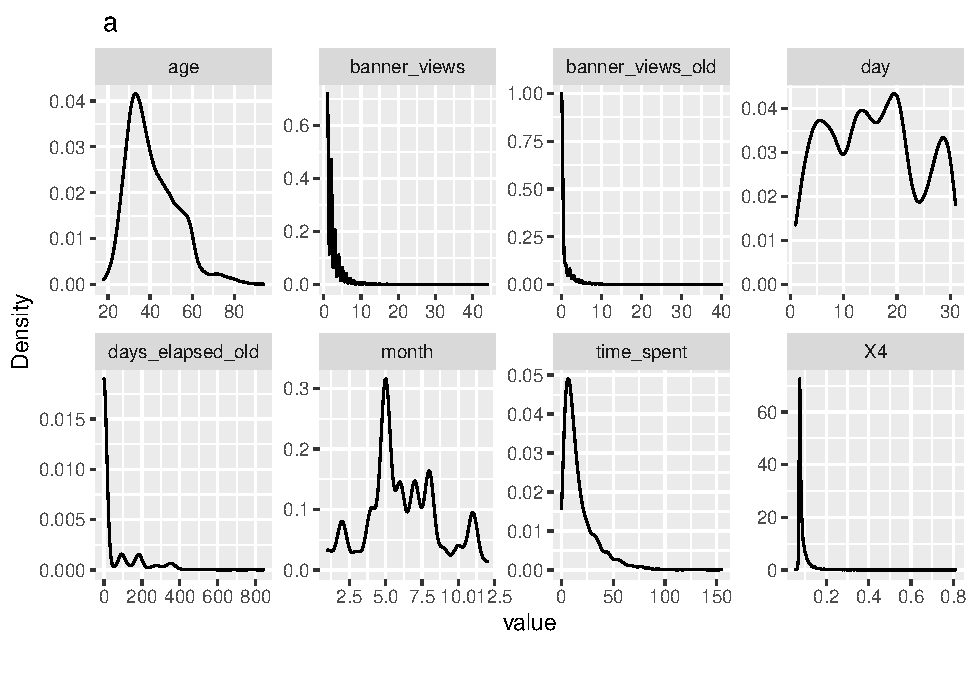
\includegraphics[width=0.75\linewidth]{report_files/figure-latex/Continous variables-6} 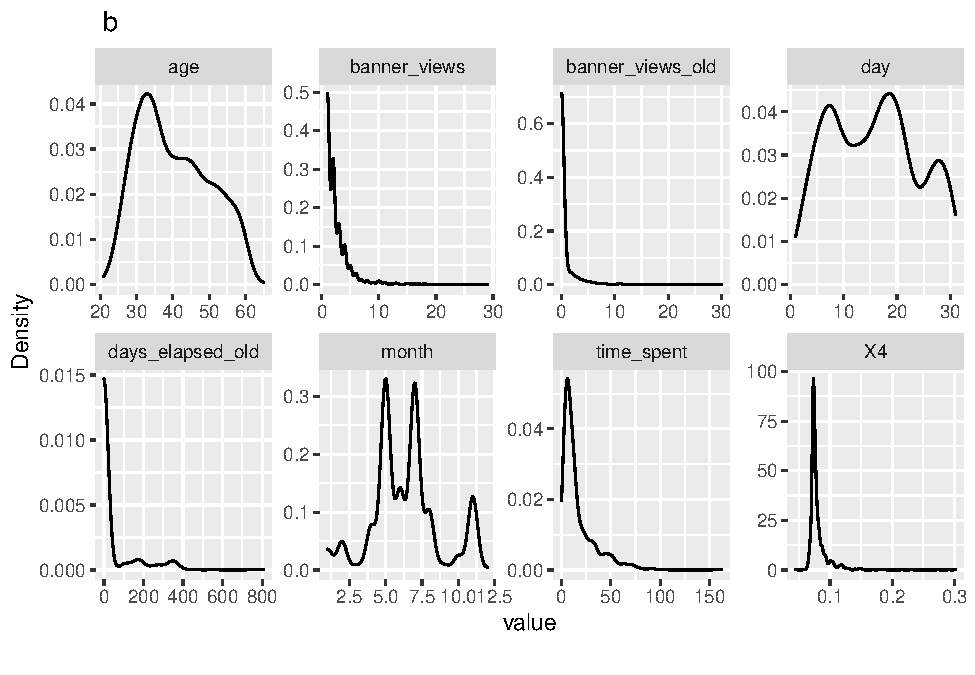
\includegraphics[width=0.75\linewidth]{report_files/figure-latex/Continous variables-7} 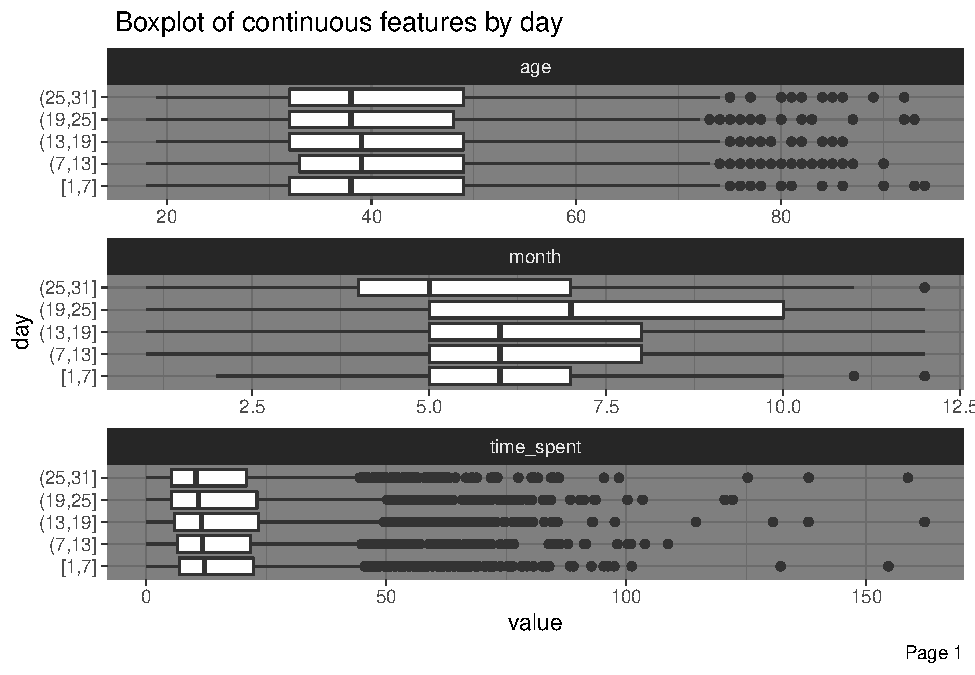
\includegraphics[width=0.75\linewidth]{report_files/figure-latex/Continous variables-8} 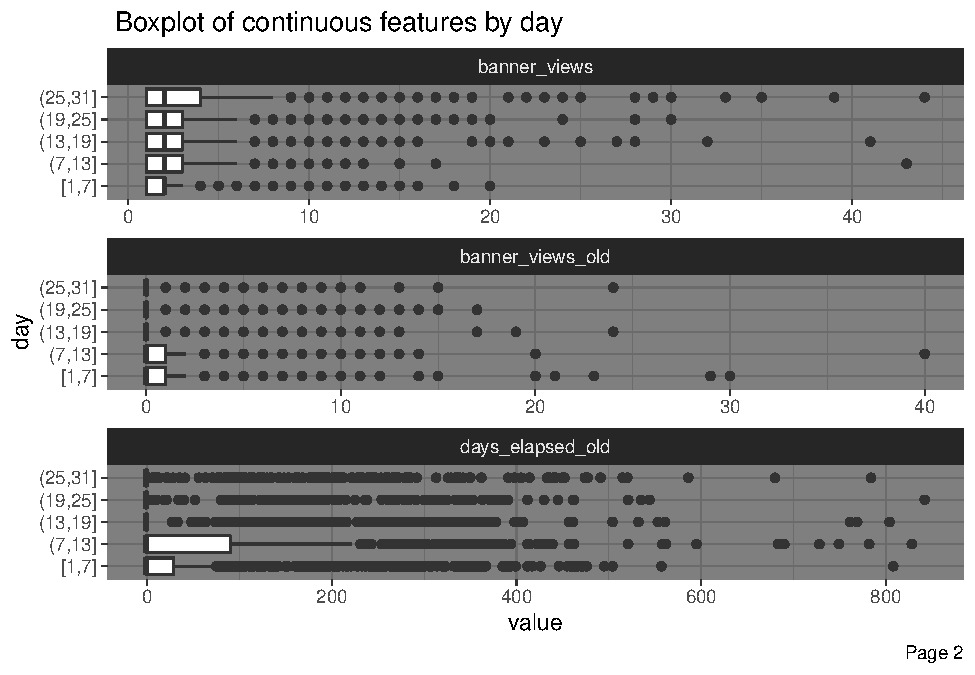
\includegraphics[width=0.75\linewidth]{report_files/figure-latex/Continous variables-9} 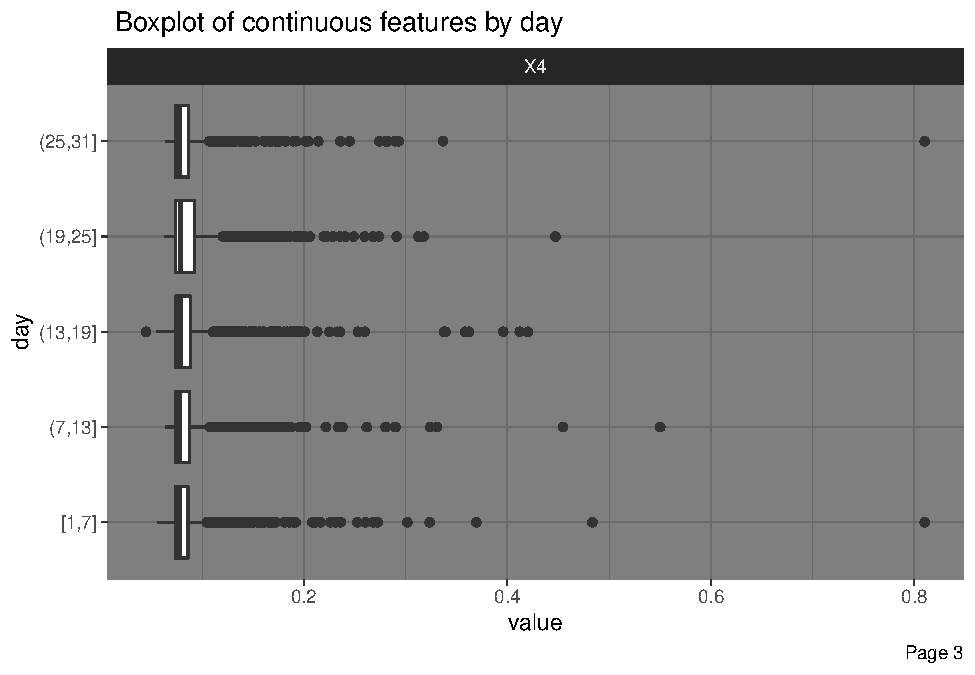
\includegraphics[width=0.75\linewidth]{report_files/figure-latex/Continous variables-10} 

}

\caption{Continous Variables}\label{fig:Continous variables}
\end{figure}
\subsection{Correlation Plot}

\subsection{EDA for Categorical}

For more sophisticated graphs, that span over multiple pages, see
function \texttt{ggarrange()} from \texttt{ggpubr} package (see
\href{http://www.sthda.com/english/articles/24-ggpubr-publication-ready-plots/81-ggplot2-easy-way-to-mix-multiple-graphs-on-the-same-page/}{link}).

For good-looking colors, have a look at the Paul Tol's palette
\url{https://personal.sron.nl/~pault/}.

\subsection{Tables}

To display a table, look at the \texttt{kable()} function from
\texttt{knitr} package. Also, consider the \texttt{kableExtra} package
for more sophisticated options (see
\href{https://haozhu233.github.io/kableExtra/awesome_table_in_pdf.pdf}{link}).
In Table \ref{tab:tblname}, we show an example that uses both
\texttt{kable} and \texttt{kableExtra}.

You can reference a table by putting the code
\texttt{\textbackslash{}\textbackslash{}label\{tab:tblname\}} inside the
caption. See code below. Then, you see that the reference works (see
Table \ref{tab:tblname}).

\begin{Shaded}
\begin{Highlighting}[]
\CommentTok{# Prepare data to put in the table}
\NormalTok{dat2 <-}\StringTok{ }\NormalTok{mtcars }\OperatorTok\StringTok{ }
\StringTok{  }\KeywordTok{group_by}\NormalTok{(cyl) }\OperatorTok\StringTok{ }
\StringTok{  }\KeywordTok{summarise}\NormalTok{(}\DataTypeTok{Average =} \KeywordTok{mean}\NormalTok{(mpg), }\DataTypeTok{Max =} \KeywordTok{max}\NormalTok{(mpg), }\DataTypeTok{Sqrt =} \KeywordTok{sum}\NormalTok{(}\KeywordTok{sqrt}\NormalTok{(mpg)))}

\CommentTok{# Print table}
\NormalTok{capt <-}\StringTok{ }\KeywordTok{paste}\NormalTok{(}\StringTok{"}\CharTok{\textbackslash{}\textbackslash{}}\StringTok{label\{tab:tblname\}Average and "}\NormalTok{,}
              \StringTok{"maximum miles per gallon for each number of cylindyers class."}\NormalTok{)}
\KeywordTok{kable}\NormalTok{(dat2,}
      \DataTypeTok{format =} \StringTok{"latex"}\NormalTok{,}
      \DataTypeTok{longtable =}\NormalTok{ F,}
      \DataTypeTok{booktabs =}\NormalTok{ T,}
      \DataTypeTok{digits =} \DecValTok{2}\NormalTok{,}
      \DataTypeTok{caption =}\NormalTok{ capt) }\OperatorTok\StringTok{ }
\StringTok{  }\KeywordTok{kable_styling}\NormalTok{(}\DataTypeTok{latex_options =} \KeywordTok{c}\NormalTok{(}\StringTok{"striped"}\NormalTok{, }\StringTok{"hold_position"}\NormalTok{))}
\end{Highlighting}
\end{Shaded}

\begin{table}[!h]

\caption{\label{tab:table1}\label{tab:tblname}Average and  maximum miles per gallon for each number of cylindyers class.}
\centering
\begin{tabular}[t]{rrrr}
\toprule
cyl & Average & Max & Sqrt\\
\midrule
\rowcolor{gray!6}  4 & 26.66 & 33.9 & 56.62\\
6 & 19.74 & 21.4 & 31.08\\
\rowcolor{gray!6}  8 & 15.10 & 19.2 & 54.21\\
\bottomrule
\end{tabular}
\end{table}

If you want to manually insert the values in the table, you can do it,
too (see Table \ref{tab:tab2}).

\begin{table}[H]
\caption{\label{tab:tab2}Number of different levels and the number of predictors that have this amount of levels.}
\centering
\begin{tabular}{lcccc}
\toprule
 & Col 1 & Col 2 & Col 3 & Col 4\\
\midrule
\rowcolor{gray!6}
Number of different values & 2 & 4 & 12 & $> 300$\\
Number of predictors & ... & ... & ... & ...\\
\bottomrule
\end{tabular}
\end{table}

\section{Models}

\subsection{Random Forest}

Out of the box, random forest method provided us with a very good
training as well as prediction accuracy on our current dataset.
Therefore, the first approach was to fit a random forest model, which
calculated its mean square error using the following formula. \[
  MSE = 1/n \sum_{i=1}^n (fi-yi)^2,
\] where n is number of data points \(fi\) is the factor prediction made
by the model and \(yi\) is the actual factor value.

We carried out cross validation for the same by using a 10 fold
cross-validation.

\subsection{Implementation}

\begin{verbatim}
## [1] "=====================================Random Forest====================================="
\end{verbatim}

\begin{verbatim}
## Confusion Matrix and Statistics
## 
##    y_pred
##        0    1
##   0 1082  158
##   1  122  770
##                                           
##                Accuracy : 0.8687          
##                  95% CI : (0.8536, 0.8827)
##     No Information Rate : 0.5647          
##     P-Value [Acc > NIR] : < 2e-16         
##                                           
##                   Kappa : 0.7317          
##                                           
##  Mcnemar's Test P-Value : 0.03647         
##                                           
##             Sensitivity : 0.8987          
##             Specificity : 0.8297          
##          Pos Pred Value : 0.8726          
##          Neg Pred Value : 0.8632          
##              Prevalence : 0.5647          
##          Detection Rate : 0.5075          
##    Detection Prevalence : 0.5816          
##       Balanced Accuracy : 0.8642          
##                                           
##        'Positive' Class : 0               
## 
\end{verbatim}

We fit several different linear models to find the positive or negative
depdendency as well as significance of each variable with respect to
\(y\). We then used them in order to reduce the number of levels in the
factor in order to improve the model further. Using this we were able to
get around \(86.87%
\) training accuracy and \(86.557%
\) for the test set.

\subsection{Random Forest Plot}

\begin{center}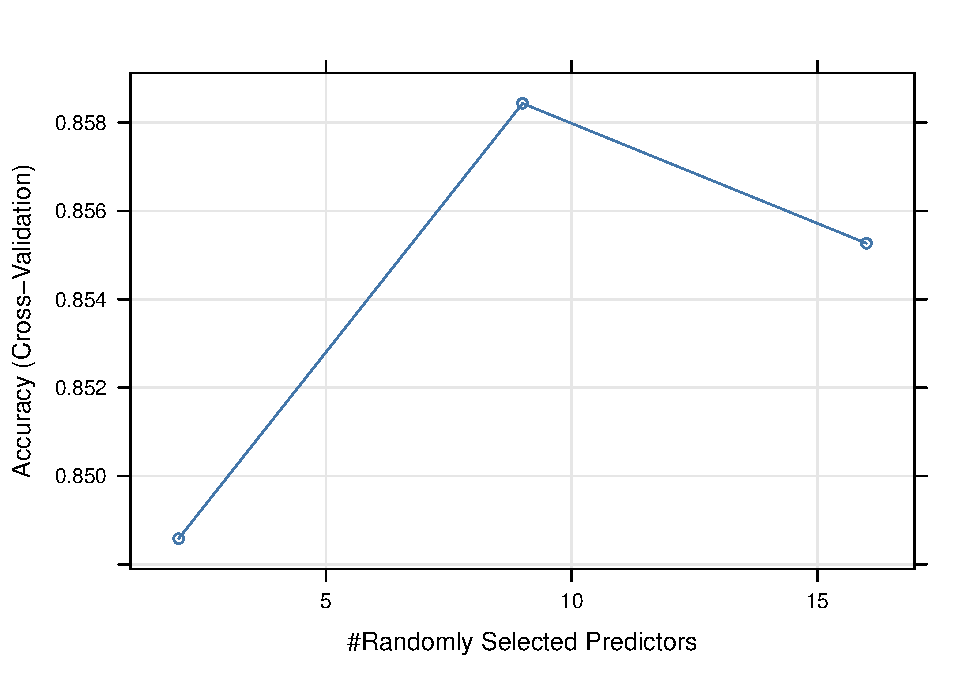
\includegraphics[width=0.75\linewidth]{report_files/figure-latex/Accuracy-1} \end{center}
\subsection{GBM Implementation}

\begin{Shaded}
\begin{Highlighting}[]
\CommentTok{#====================================================================================================}
\KeywordTok{rm}\NormalTok{(}\DataTypeTok{list=}\KeywordTok{ls}\NormalTok{())}
\CommentTok{#GBM to find most relevant variables}
\KeywordTok{library}\NormalTok{(}\StringTok{"gbm"}\NormalTok{)}
\KeywordTok{set.seed}\NormalTok{(}\DecValTok{77850}\NormalTok{)}
\NormalTok{dataset <-}\StringTok{ }\KeywordTok{read.csv}\NormalTok{(}\StringTok{'train.csv'}\NormalTok{)}
\NormalTok{gbm.fit <-}\StringTok{ }\KeywordTok{gbm}\NormalTok{(y}\OperatorTok{~}\NormalTok{.,}
               \DataTypeTok{distribution=}\StringTok{"bernoulli"}\NormalTok{,}
               \DataTypeTok{data=}\NormalTok{dataset,}
               \DataTypeTok{n.trees=}\DecValTok{750}\NormalTok{,}
               \DataTypeTok{interaction.depth=}\DecValTok{4}\NormalTok{,}
               \DataTypeTok{shrinkage=}\FloatTok{0.01}\NormalTok{,}\DataTypeTok{cv.folds =} \DecValTok{3}\NormalTok{)}

\KeywordTok{summary}\NormalTok{(gbm.fit)}
\end{Highlighting}
\end{Shaded}

\begin{verbatim}
##                               var    rel.inf
## time_spent             time_spent 49.6997337
## outcome_old           outcome_old 14.8535040
## month                       month  8.6110871
## device                     device  7.2223816
## X3                             X3  5.4987384
## age                           age  3.6024227
## days_elapsed_old days_elapsed_old  2.9312266
## day                           day  2.1541162
## job                           job  1.5040134
## banner_views         banner_views  1.3335633
## X4                             X4  1.2479805
## X1                             X1  0.4514397
## education               education  0.3257785
## banner_views_old banner_views_old  0.3055869
## marital                   marital  0.2584273
## X2                             X2  0.0000000
\end{verbatim}

\begin{center}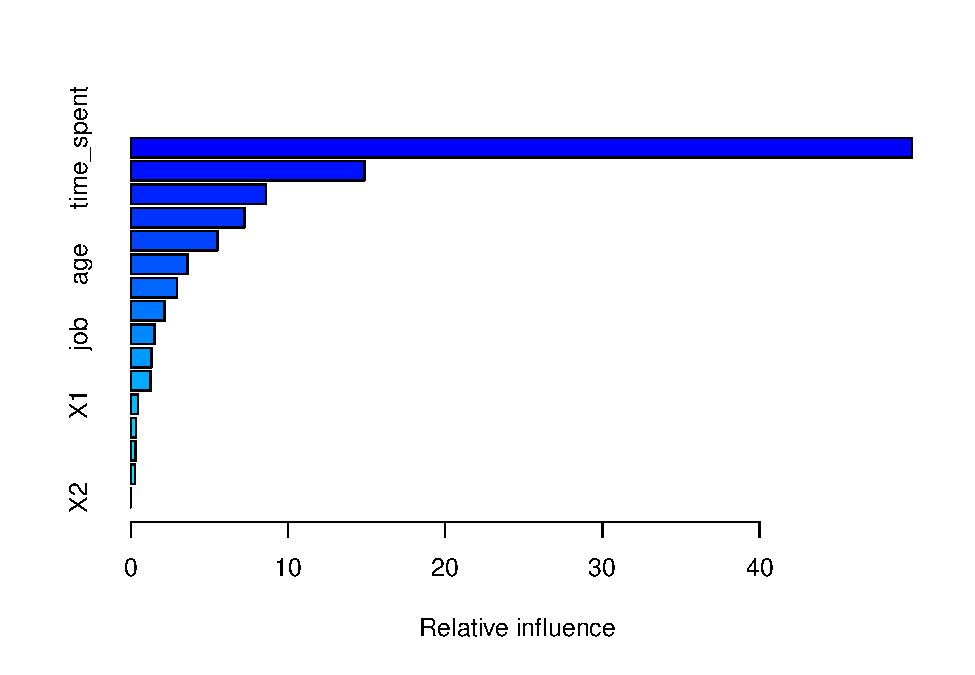
\includegraphics[width=0.75\linewidth]{report_files/figure-latex/unnamed-chunk-1-1} \end{center}
\section{C5.0 Implementation}

While implementing several models, a good prediction accuracy was also
observed in case of C5.0 and got a prediction accuracy of \(87.15%
\) over the given dataset.

\begin{verbatim}
## [1] "=====================================Random Forest====================================="
\end{verbatim}

\begin{verbatim}
## Confusion Matrix and Statistics
## 
##    y_pred
##        0    1
##   0 1098  142
##   1  132  760
##                                           
##                Accuracy : 0.8715          
##                  95% CI : (0.8565, 0.8854)
##     No Information Rate : 0.5769          
##     P-Value [Acc > NIR] : <2e-16          
##                                           
##                   Kappa : 0.7363          
##                                           
##  Mcnemar's Test P-Value : 0.5866          
##                                           
##             Sensitivity : 0.8927          
##             Specificity : 0.8426          
##          Pos Pred Value : 0.8855          
##          Neg Pred Value : 0.8520          
##              Prevalence : 0.5769          
##          Detection Rate : 0.5150          
##    Detection Prevalence : 0.5816          
##       Balanced Accuracy : 0.8676          
##                                           
##        'Positive' Class : 0               
## 
\end{verbatim}

\begin{center}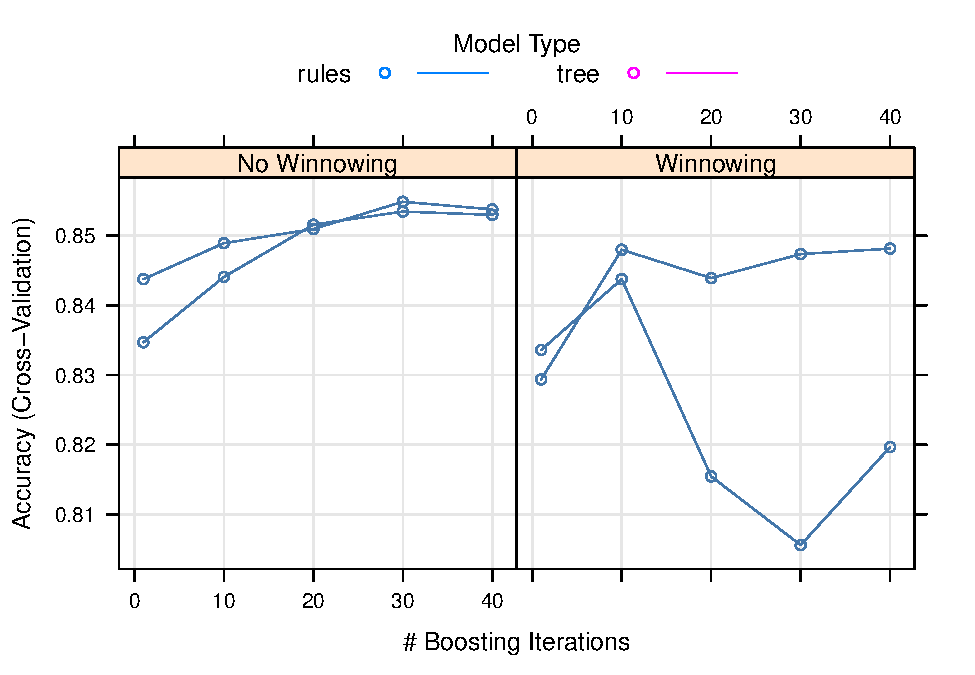
\includegraphics[width=0.75\linewidth]{report_files/figure-latex/unnamed-chunk-2-1} \end{center}
\section{Results}

We obtained the best prediction accuracy from the C5.0 model followed by
Random forest where we carried out data manipulation by decreasing the
number of factor levels.

\section{Tests}
\subsection{Preliminary Implementation}

We started by dividing the set into 75-35 percent split and running them
through different machine learning models in a crude manner to check out
of the box which model tends to perform best on the given dataset.
\emph{Support Vector Machine}

\begin{verbatim}
## [1] "======================================SVM====================================="
\end{verbatim}

\begin{verbatim}
## Confusion Matrix and Statistics
## 
##    y_pred
##        0    1
##   0 1083  157
##   1  168  724
##                                           
##                Accuracy : 0.8476          
##                  95% CI : (0.8316, 0.8626)
##     No Information Rate : 0.5868          
##     P-Value [Acc > NIR] : <2e-16          
##                                           
##                   Kappa : 0.6862          
##                                           
##  Mcnemar's Test P-Value : 0.5791          
##                                           
##             Sensitivity : 0.8657          
##             Specificity : 0.8218          
##          Pos Pred Value : 0.8734          
##          Neg Pred Value : 0.8117          
##              Prevalence : 0.5868          
##          Detection Rate : 0.5080          
##    Detection Prevalence : 0.5816          
##       Balanced Accuracy : 0.8438          
##                                           
##        'Positive' Class : 0               
## 
\end{verbatim}

\emph{Random Forest Classification}

\begin{verbatim}
## [1] "=====================================Random Forest====================================="
\end{verbatim}

\begin{verbatim}
## Confusion Matrix and Statistics
## 
##    y_pred
##        0    1
##   0 1092  148
##   1  144  748
##                                           
##                Accuracy : 0.863           
##                  95% CI : (0.8477, 0.8774)
##     No Information Rate : 0.5797          
##     P-Value [Acc > NIR] : <2e-16          
##                                           
##                   Kappa : 0.7188          
##                                           
##  Mcnemar's Test P-Value : 0.8606          
##                                           
##             Sensitivity : 0.8835          
##             Specificity : 0.8348          
##          Pos Pred Value : 0.8806          
##          Neg Pred Value : 0.8386          
##              Prevalence : 0.5797          
##          Detection Rate : 0.5122          
##    Detection Prevalence : 0.5816          
##       Balanced Accuracy : 0.8592          
##                                           
##        'Positive' Class : 0               
## 
\end{verbatim}

\emph{Logistic Regression}

\begin{verbatim}
## [1] "=====================================Logistic Regression====================================="
\end{verbatim}

\begin{verbatim}
## Confusion Matrix and Statistics
## 
##    y_pred
##        0    1
##   0 1110  130
##   1  257  635
##                                           
##                Accuracy : 0.8185          
##                  95% CI : (0.8015, 0.8346)
##     No Information Rate : 0.6412          
##     P-Value [Acc > NIR] : < 2.2e-16       
##                                           
##                   Kappa : 0.6194          
##                                           
##  Mcnemar's Test P-Value : 1.504e-10       
##                                           
##             Sensitivity : 0.8120          
##             Specificity : 0.8301          
##          Pos Pred Value : 0.8952          
##          Neg Pred Value : 0.7119          
##              Prevalence : 0.6412          
##          Detection Rate : 0.5206          
##    Detection Prevalence : 0.5816          
##       Balanced Accuracy : 0.8210          
##                                           
##        'Positive' Class : 0               
## 
\end{verbatim}

\emph{Naive Bayes}

\begin{verbatim}
## [1] "=====================================Naive Bayes====================================="
\end{verbatim}

\begin{verbatim}
## Confusion Matrix and Statistics
## 
##    y_pred
##        0    1
##   0 1020  220
##   1  325  567
##                                           
##                Accuracy : 0.7444          
##                  95% CI : (0.7253, 0.7628)
##     No Information Rate : 0.6309          
##     P-Value [Acc > NIR] : < 2.2e-16       
##                                           
##                   Kappa : 0.4659          
##                                           
##  Mcnemar's Test P-Value : 8.394e-06       
##                                           
##             Sensitivity : 0.7584          
##             Specificity : 0.7205          
##          Pos Pred Value : 0.8226          
##          Neg Pred Value : 0.6357          
##              Prevalence : 0.6309          
##          Detection Rate : 0.4784          
##    Detection Prevalence : 0.5816          
##       Balanced Accuracy : 0.7394          
##                                           
##        'Positive' Class : 0               
## 
\end{verbatim}

\emph{Decision Tree}

\begin{verbatim}
## [1] "=====================================Decision Trees====================================="
\end{verbatim}

\begin{verbatim}
## Confusion Matrix and Statistics
## 
##    y_pred
##        0    1
##   0 1064  176
##   1  262  630
##                                           
##                Accuracy : 0.7946          
##                  95% CI : (0.7768, 0.8115)
##     No Information Rate : 0.622           
##     P-Value [Acc > NIR] : < 2.2e-16       
##                                           
##                   Kappa : 0.5721          
##                                           
##  Mcnemar's Test P-Value : 4.877e-05       
##                                           
##             Sensitivity : 0.8024          
##             Specificity : 0.7816          
##          Pos Pred Value : 0.8581          
##          Neg Pred Value : 0.7063          
##              Prevalence : 0.6220          
##          Detection Rate : 0.4991          
##    Detection Prevalence : 0.5816          
##       Balanced Accuracy : 0.7920          
##                                           
##        'Positive' Class : 0               
## 
\end{verbatim}

\emph{kNN}

\begin{verbatim}
## [1] "=====================================KNN====================================="
\end{verbatim}

\begin{verbatim}
## Confusion Matrix and Statistics
## 
##    y_pred
##        0    1
##   0 1107  133
##   1  282  610
##                                          
##                Accuracy : 0.8053         
##                  95% CI : (0.7879, 0.822)
##     No Information Rate : 0.6515         
##     P-Value [Acc > NIR] : < 2.2e-16      
##                                          
##                   Kappa : 0.5904         
##                                          
##  Mcnemar's Test P-Value : 3.729e-13      
##                                          
##             Sensitivity : 0.7970         
##             Specificity : 0.8210         
##          Pos Pred Value : 0.8927         
##          Neg Pred Value : 0.6839         
##              Prevalence : 0.6515         
##          Detection Rate : 0.5192         
##    Detection Prevalence : 0.5816         
##       Balanced Accuracy : 0.8090         
##                                          
##        'Positive' Class : 0              
## 
\end{verbatim}

\section{Lasso, Ridge and ElasticNet Implementation}

This is presently something we are carrying out in order to identify a
good fit for the model. Here, \(nfolds\)=10 (Number of Folds)

\begin{verbatim}
## [1] "Ridge Implementation"
\end{verbatim}

\begin{verbatim}
## [1] "Testing Accuracy"
\end{verbatim}

\begin{verbatim}
## [1] 0.8184803
\end{verbatim}

\begin{verbatim}
## [1] "Training Accuracy"
\end{verbatim}

\begin{verbatim}
## [1] 0.8110729
\end{verbatim}

\begin{verbatim}
## [1] "ElasticNet Implementation"
\end{verbatim}

\begin{verbatim}
## [1] "Testing Accuracy"
\end{verbatim}

\begin{verbatim}
## [1] 0.8245779
\end{verbatim}

\begin{verbatim}
## [1] "Training Accuracy"
\end{verbatim}

\begin{verbatim}
## [1] 0.8148264
\end{verbatim}

\begin{verbatim}
## [1] "Lasso Implementation"
\end{verbatim}

\begin{verbatim}
## [1] "Testing Accuracy"
\end{verbatim}

\begin{verbatim}
## [1] 0.8236398
\end{verbatim}

\begin{verbatim}
## [1] "Training Accuracy"
\end{verbatim}

\begin{verbatim}
## [1] 0.8143572
\end{verbatim}

\begin{center}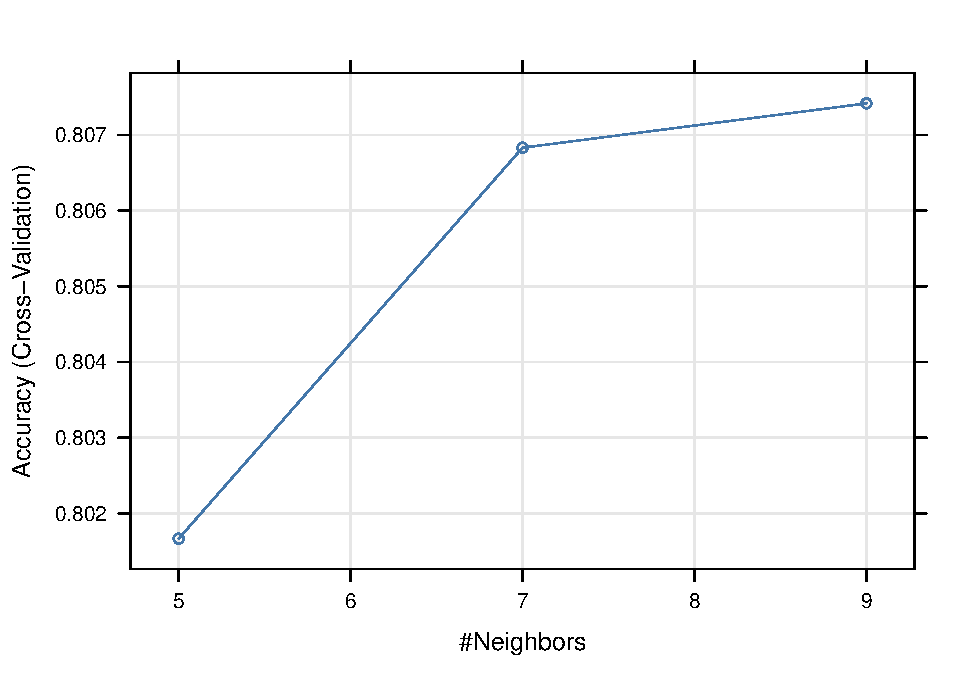
\includegraphics[width=0.75\linewidth]{report_files/figure-latex/unnamed-chunk-9-1} 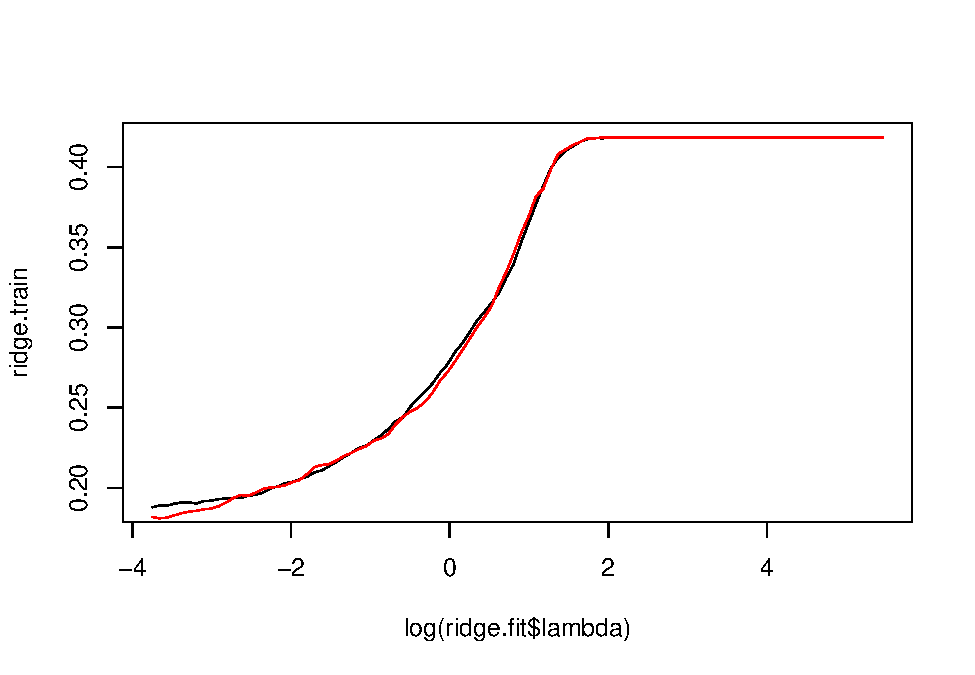
\includegraphics[width=0.75\linewidth]{report_files/figure-latex/unnamed-chunk-9-2} 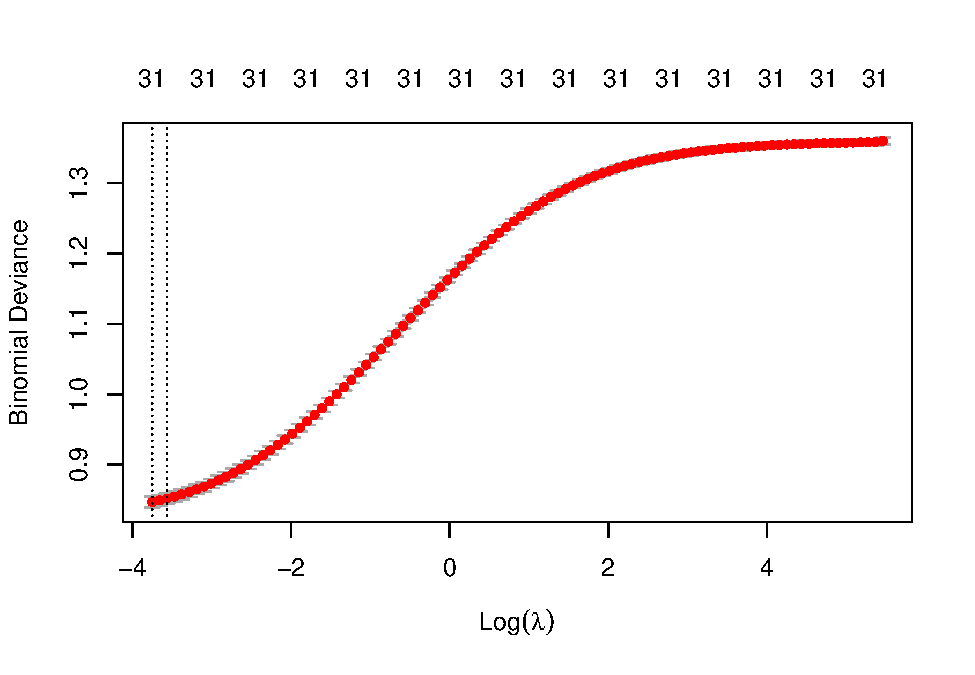
\includegraphics[width=0.75\linewidth]{report_files/figure-latex/unnamed-chunk-9-3} 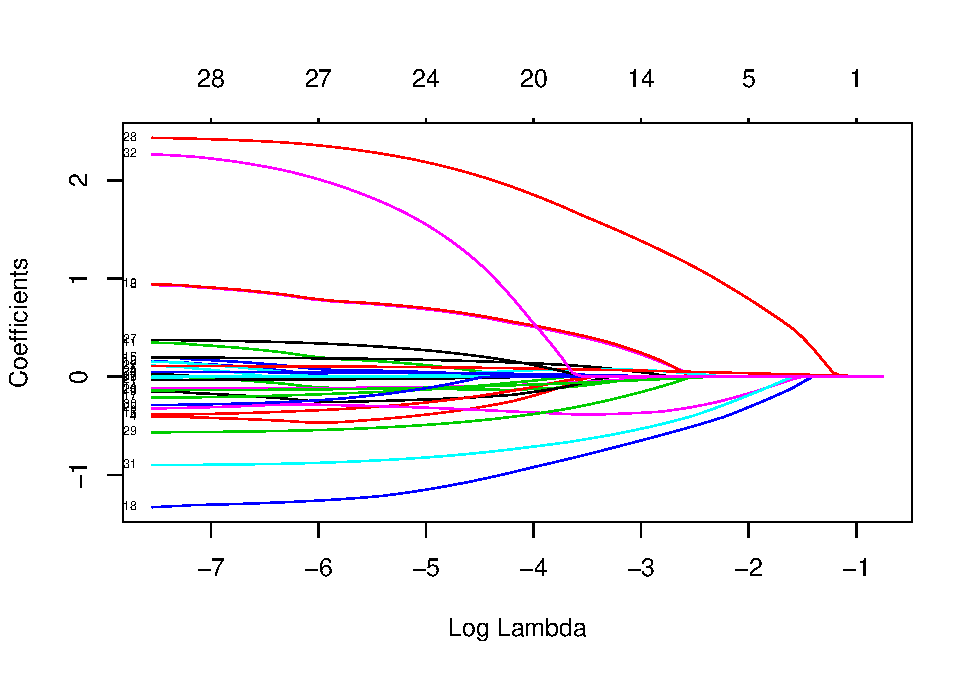
\includegraphics[width=0.75\linewidth]{report_files/figure-latex/unnamed-chunk-9-4} 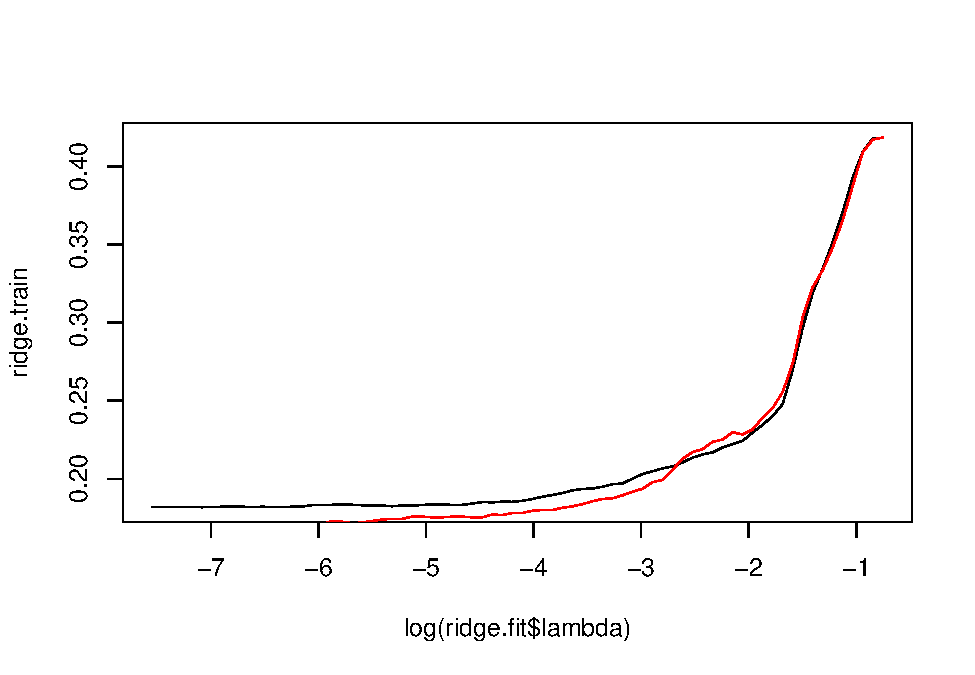
\includegraphics[width=0.75\linewidth]{report_files/figure-latex/unnamed-chunk-9-5} 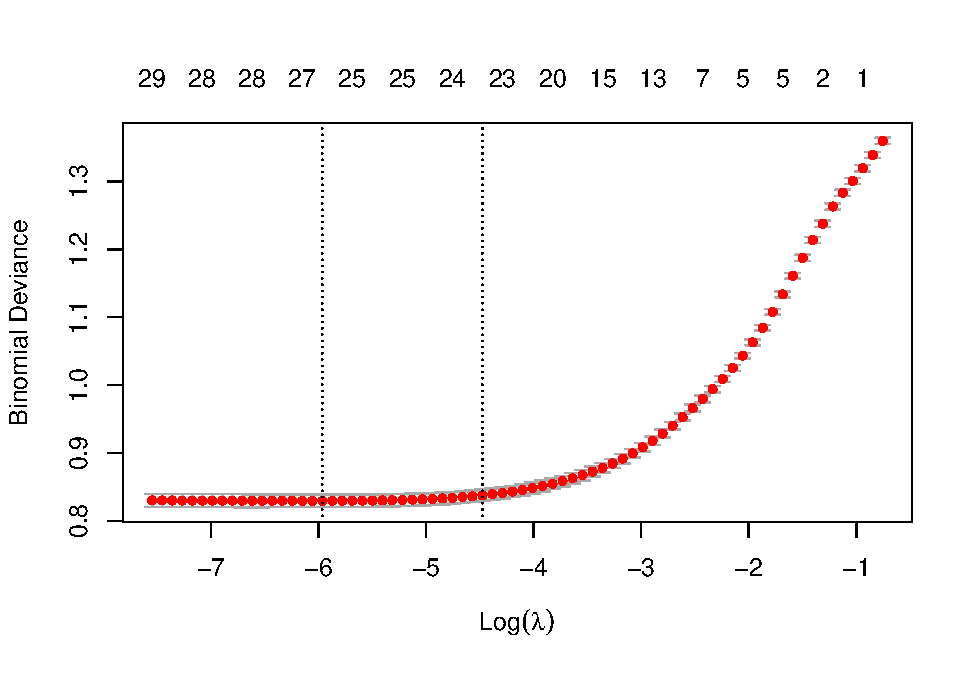
\includegraphics[width=0.75\linewidth]{report_files/figure-latex/unnamed-chunk-9-6} 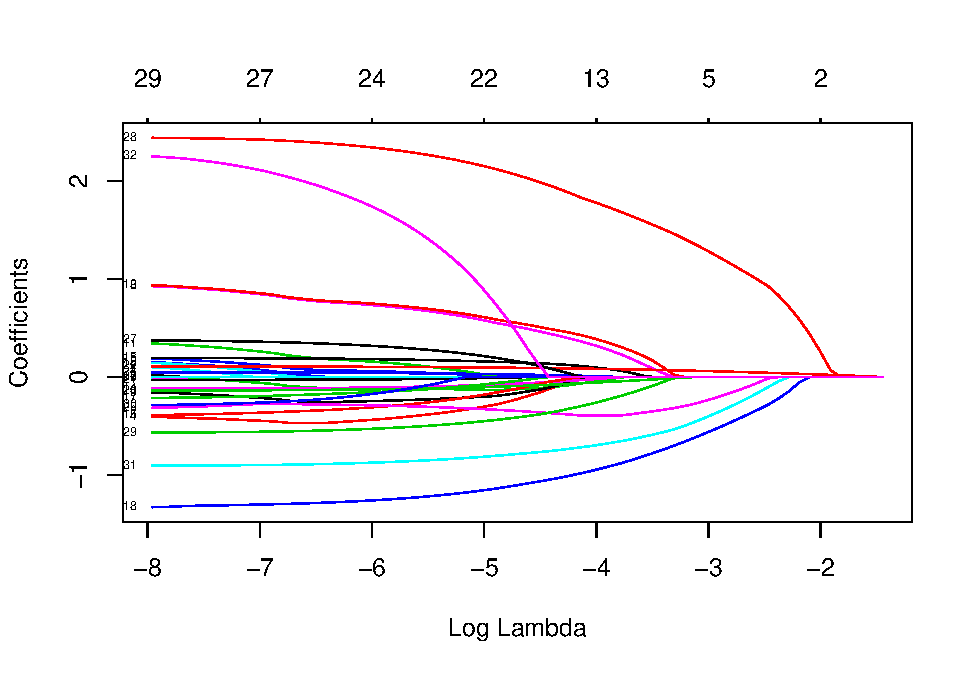
\includegraphics[width=0.75\linewidth]{report_files/figure-latex/unnamed-chunk-9-7} 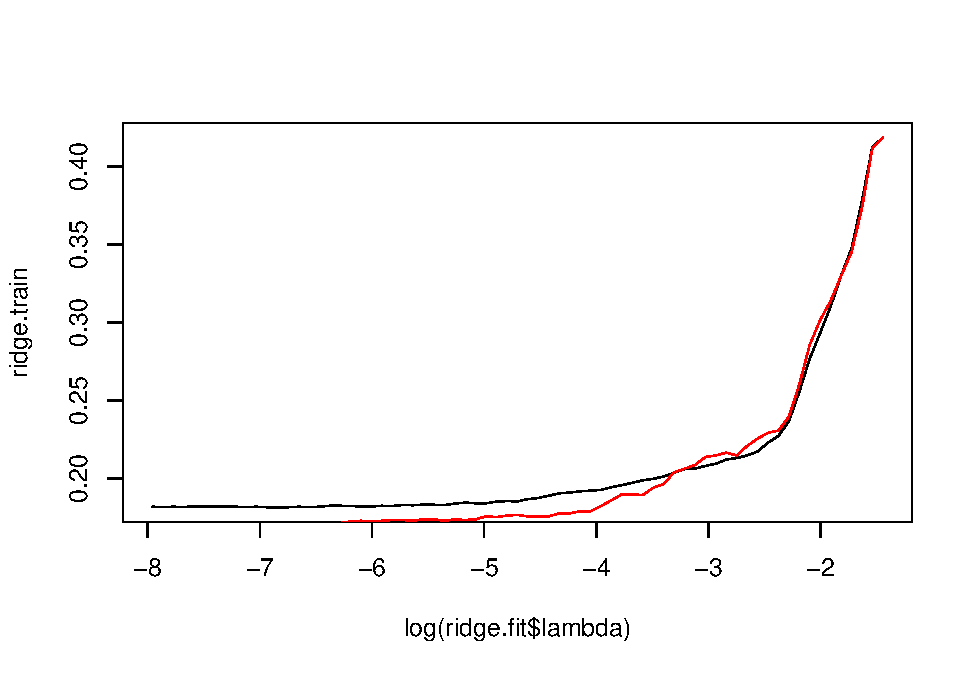
\includegraphics[width=0.75\linewidth]{report_files/figure-latex/unnamed-chunk-9-8} 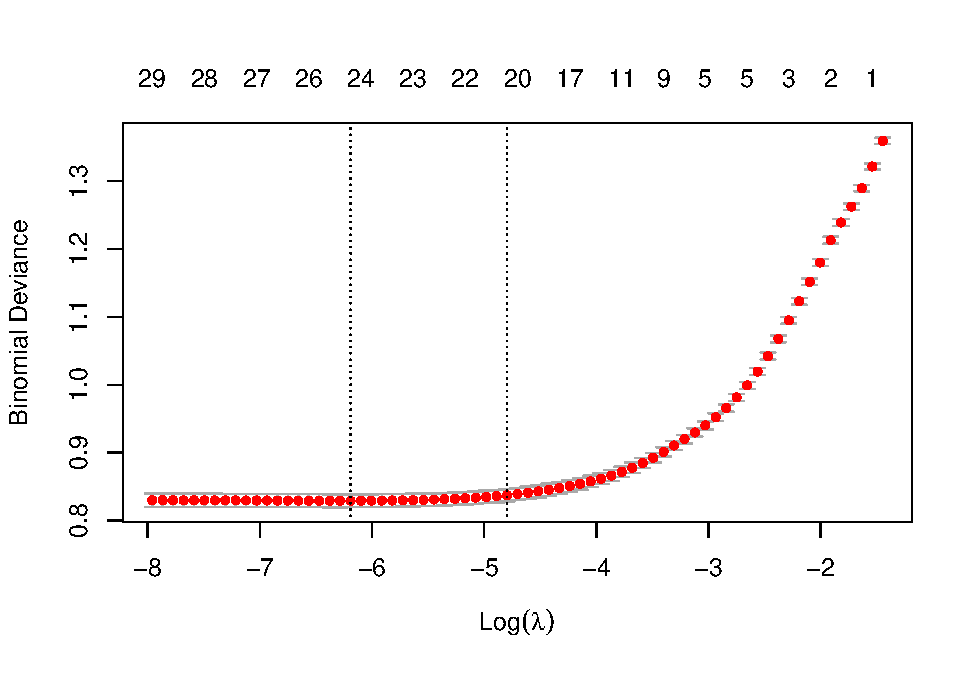
\includegraphics[width=0.75\linewidth]{report_files/figure-latex/unnamed-chunk-9-9} \end{center}
\section{Detailed kNN implementation}

\begin{Shaded}
\begin{Highlighting}[]
\CommentTok{#===============================================================================================================================}
\CommentTok{#Accuracy of the KNN model at different k values}
\KeywordTok{rm}\NormalTok{(}\DataTypeTok{list=}\KeywordTok{ls}\NormalTok{())}
\KeywordTok{library}\NormalTok{(caret)}
\KeywordTok{set.seed}\NormalTok{(}\DecValTok{123}\NormalTok{)}
\NormalTok{classSim <-}\StringTok{ }\KeywordTok{read.csv}\NormalTok{(}\StringTok{'train.csv'}\NormalTok{)}
\NormalTok{classSim}\OperatorTok{$}\NormalTok{y =}\StringTok{ }\KeywordTok{factor}\NormalTok{(classSim}\OperatorTok{$}\NormalTok{y, }\DataTypeTok{levels =} \KeywordTok{c}\NormalTok{(}\DecValTok{0}\NormalTok{, }\DecValTok{1}\NormalTok{))}

\NormalTok{nfolds <-}\StringTok{ }\DecValTok{10}
\NormalTok{trControl <-}\StringTok{ }\KeywordTok{trainControl}\NormalTok{(}\DataTypeTok{method  =} \StringTok{"cv"}\NormalTok{,}
                          \DataTypeTok{number  =}\NormalTok{ nfolds)}
\NormalTok{max_k <-}\StringTok{ }\DecValTok{100}

\CommentTok{#Use this function to plot graphs for all the possible models used}
\NormalTok{fit <-}\StringTok{ }\KeywordTok{train}\NormalTok{(}\DataTypeTok{form =}\NormalTok{ y }\OperatorTok{~}\StringTok{ }\NormalTok{.,}
             \DataTypeTok{data =}\NormalTok{ classSim,}
             \DataTypeTok{method     =} \StringTok{"knn"}\NormalTok{, }\CommentTok{#can be changed here to 17 other configurations including random forest etc and accuracy can be plotted vs n trees/k value etc}
             \DataTypeTok{trControl  =}\NormalTok{ trControl,}
             \DataTypeTok{metric     =} \StringTok{"Accuracy"}\NormalTok{)}

\NormalTok{palette =}\StringTok{ }\KeywordTok{c}\NormalTok{(}\DataTypeTok{tolBlue =} \StringTok{"#4477AA"}\NormalTok{,}
            \DataTypeTok{tolRed =} \StringTok{"#EE6677"}\NormalTok{,}
            \DataTypeTok{tolGreen =} \StringTok{"#228833"}\NormalTok{,}
            \DataTypeTok{tolYellow =} \StringTok{"#CCBB44"}\NormalTok{,}
            \DataTypeTok{tolCyan =} \StringTok{"#66CCEE"}\NormalTok{,}
            \DataTypeTok{tolPurple =} \StringTok{"#AA3377"}\NormalTok{,}
            \DataTypeTok{tolGrey =} \StringTok{"#BBBBBB"}\NormalTok{) }\OperatorTok\StringTok{ }\KeywordTok{unname}\NormalTok{()}
\KeywordTok{plot}\NormalTok{(fit, }\DataTypeTok{col =}\NormalTok{ palette[}\DecValTok{1}\NormalTok{])}
\end{Highlighting}
\end{Shaded}

\begin{center}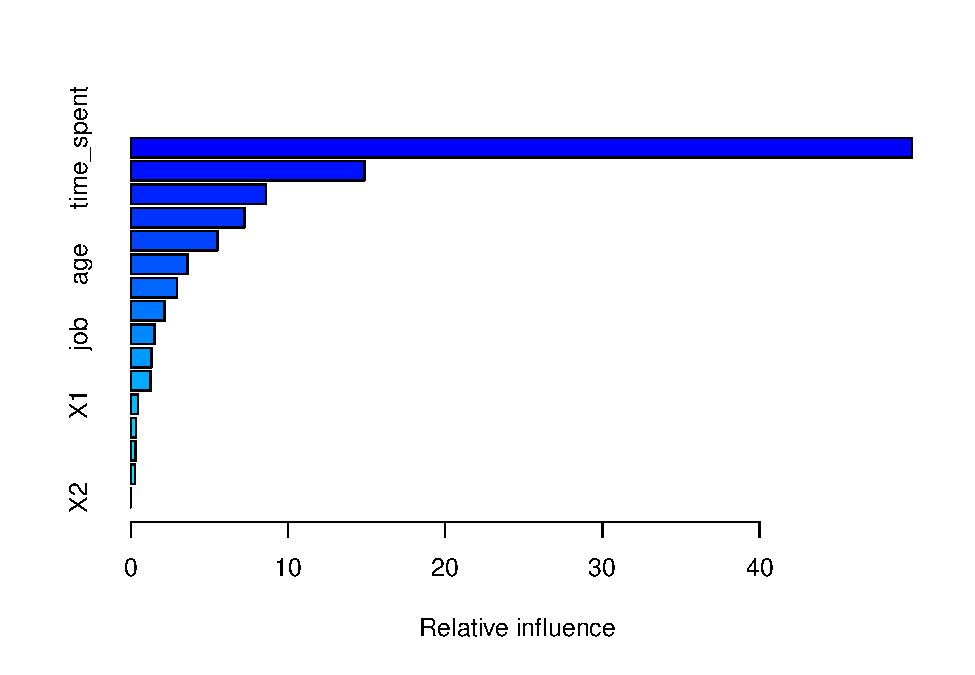
\includegraphics[width=0.75\linewidth]{report_files/figure-latex/unnamed-chunk-10-1} \end{center}

\begin{table} 
\begin{center}
\begin{tabular}{|l|c|c|c|} \hline
& Training error & CV error & Public Leaderboard error (if available)\\
  kNN & ... & ... & ...\\
  Ridge & ... & ... & ...\\
  lasso & ... & ... & ...\\
  ElasticNet & ... & ... & ... \\
  random forest & ... & ... \\
  SVM & ... & ... \\
  LDA & ... & ... \\
  QDA & ... & ... \\
  C5.0 & ... & ... \\
  
\hline
\end{tabular}
\end{center}
\caption{Training and CV error of the different models.} \label{tab_res}
\end{table}

\end{document}
